\chapter{Referencial Teórico}\label{cap:refTeor}


Para se compreender  a temática proposta  este capítulo abordará o conteúdo base deste trabalho dividido em 3 seções: Aprendizado de Máquina, Discretização e Trabalhos Correlatos. 

A aprendizagem de máquina utiliza métodos de inferências lógicas para aquisições de novos conhecimentos, e um dos tipos de inferência comentada nesta seção são os aprendizados indutivos, que dentre seus tipos terá o maior destaque  ao aprendizado supervisionado, foco maior dessa proposta de mestrado. ``Na aprendizagem indutiva os algoritmos podem, na melhor das hipóteses, garantir que a hipótese de saída se encaixe no conceito de destino sobre os dados de treinamento'' \cite[p.23]{Mitchell1997}.

%\epigraph{Na aprendizagem indutiva os algoritmos podem, na melhor das hipóteses, garantir que a hipótese de saída se encaixe no conceito de destino sobre os dados de treinamento. Na falta de mais informações, nossa suposição é que a melhor hipótese em relação a instâncias não vistas é a hipótese que melhor se ajusta aos dados de treinamento observados}{ \cite[p.23]{Mitchell1997}}


%No aprendizado indutivo a indução é um tipo de inferência lógica, a partir de um pequeno número de observações pode-se ter uma conclusão geral de todo o conjunto. Então, caso a pequena amostra não tenha dados suficientes ou os dados da amostra não forem relevantes, o conhecimento induzido acaba sendo prejudicado por generalizar o conhecimento adquirido, dessa amostra, para todo o grupo de dados.

Já na seção \ref{cap:refTeor:sec:discret} dissertará sobre a técnica de discretização adotada nesta pesquisa. Possuindo grande contribuição para os resultados gerados, e ganhando assim uma seção própria para explanação de como funciona essa técnica. E na seção \ref{cap:refTeor:sec:trabcorrel}, serão abordados trabalhos que possuam mesmas características desta pesquisa adicionando conhecimento ao tema.



\section{Aprendizado de Máquina}\label{cap:refTeor:sec:aprendMaq}

 A aprendizagem de máquina, diferente das metodologias tradicionais de implementação, utiliza sua experiência anterior, para melhorar suas respostas a partir de problemas em determinadas áreas. 
 
 ``Um programa de computador aprende com a experiência E em relação a alguma classe de tarefas T e medida de desempenho P, se seu desempenho em tarefas em T, conforme medido por P, melhora com a experiência E'' \cite[p. 2]{Mitchell1997}. 
 
 %\newtheorem{defaprendmaq}{Definição}
 % \begin{teorema}
 %  Um programa de computador aprende com a experiência E em relação a alguma classe de tarefas T e medida de desempenho P, se seu desempenho em tarefas em T, conforme medido por P, melhora com a experiência E
 %  \label{teo:defaprendmaq}
 % \end{teorema}
 
Para melhor explicar a citação acima, destaca-se o determinado exemplo: considerar o reconhecimento facial de uma pessoa utilizando aprendizado de máquina. Então caso fossem  inseridas várias fotos tituladas de uma certa pessoa (T) no banco de dados, e após vários exemplos (E), fotos dessa pessoa, o programa de computador seria capaz de predizer (P) se uma nova foto, ainda não inserida no banco de dados, seria dessa  determinada pessoa através de aprendizado  anterior (E), ou melhor, de fotos que foram anteriormente inseridas.

O aprendizado de máquina seriam algoritmos capazes de ``aprender'' automaticamente através de  determinados exemplos, ou comportamentos. Esse ``aprendizado'' automático preenche algumas lacunas no desenvolvimento de programas, posto que não é possível simplesmente exigir do projetista implementar melhorias em um sistema, de forma que ele esteja robusto bastante para lidar com todas as situações \cite{RusselStuart.Norvig2013}, pois seria impossível um programador antecipar todas as situações possíveis de implementação.


%Alguns motivos justificam que não é possível simplesmente exigir do projetista implementar melhorias no sistema, de forma que ele esteja robusto bastante para lidar com todas as situações \cite{RusselStuart.Norvig2013}. Um  desses motivos seria a incapacidade da antecipação de todas as situações possíveis de implementação por parte do programador. Fazendo um resumo, aprendizado de máquina seriam algoritmos capazes de aprender automaticamente através de  determinados exemplos, ou comportamentos. 

Utilizando a idéia do exemplo anterior, uma vez inserida uma foto no banco de dados e determiná-la como masculina, nesse momento, estará se fazendo uma classificação desse novo registro (nova foto). Uma vez com a base de dados classificada, pode-se utilizar algoritmos para predizer um novo registro e defini-lo como masculino ou feminino. Predizer uma determinada condição irá depender da base de dados como também do algoritmo utilizado para fazer essa classificação. Alguns  exemplos de algoritmos são:  redes neurais, árvores de decisão, Suport Vector Machine – SVM, etc. A escolha apropriada do algoritmo se dará através de métricas que avaliarão o desempenho de cada um, e a melhor métrica, será o algoritmo apropriado para aquele problema de classificação de dados. 

%A partir desta síntese, tem-se uma observação. A classificação de dados no contexto de aprendizado de máquina, são compostos por dois pilares. Um, seriam os \textbf{dados} a serem classificados, e outro, o \textbf{algoritmo} que irá atuar nessa base de dados. Existem vários algoritmos como exemplo: redes neurais, árvores de decisão, Suport Vector Machine – SVM, etc. Qualquer um destes algoritmos são utilizados para encontrar um classificador. E a escolha apropriada se dará através de métricas que avaliarão o desempenho de cada um, e a melhor métrica, será o algoritmo apropriado para aquele problema de classificação de dados. 

Em aprendizado de máquina são vários os cenários encontrados, e segundo \citeonline{Mohri2012} são eles: aprendizado supervisionado, aprendizado não-supervisionado, aprendizado semi-supervisionado, aprendizado por reforço e  muitos outros cenários intermediários e um pouco mais complexos podem existir. Todavia nesta pesquisa será comentado alguns cenários de referência para esse trabalho.

\subsection{Aprendizado Supervisionado}\label{cap:refTeor:ssec:aprendSup}

O estudo sobre aprendizado supervisionado é um método que através de uma base de dados classificada, será realizado uma predição de novos registros com base em vários desses exemplos já classificados, ou seja, é quando existir casos que possuem uma classificador disponível para determinados conjunto de dados (conjunto de treinamento), mas precisa ser previstos para outras instâncias. Os responsáveis por essas predições de novos registros são algoritmos de aprendizado supervisionados projetados para determinados fins.


O termo ''Supervisionado'' indica uma correlação entre os dados de entrada com a saída desejada (classe). Seguindo o padrão de exemplo anterior considere: uma base de dados de imagens de rostos, onde cada imagen possui uma saída representada por uma classe (masculino ou feminino). A tarefa seria criar um preditor capaz de acertar a cada novo registro se a imagem é masculina ou feminina. Seria  difícil  implementar de maneira tradicional, utilizando estruturas condicionais e laços, uma vez que são inúmeras as diferenças das faces masculinas e femininas. Embora haja uma dificuldade de distinção entre as faces, uma alternativa seria dar exemplos de rostos classificados, masculino ou feminino,  e através desses exemplos aplicar o algoritmo que automaticamente faça a máquina ''aprender'' uma regra para predizer qual sexo pertence cada rosto  \cite{Barber2011}.

Em \cite{RusselStuart.Norvig2013} é feito apresentação formal do funcionamento da aprendizagem supervisionada. Dado um conjunto de treinamento 
\begin{equation}
 (x_{1},y_{2}),(x_{2},y_{2}),...(x_{n},y_{n}),
 \label{eq:aprendSup}
\end{equation}
onde cada ${y_{j}} $ foi gerado por ${y=f(x)}$ desconhecida. Encontrar uma função ${h}$ que se aproxime da função ${f}$ real.

%Antes de falar dos algoritmos utilizados nesse texto, a aprendizagem supervisionada detém dois tipos de casos: regressão e classificação. A classificação, contêm variáveis com valores discretos, onde as amostras destas variáveis de saída estão na forma de categorias. Como exemplo poderia ser masculino e feminino. Já no tipo regressão, possuem valores contínuos: quantidade de água em ml, velocidade de um carro, altura de uma pessoa.

A função ${h}$ é uma hipótese onde prevê um melhor desempenho entre as hipóteses possíveis através dos conjuntos de dados, que são diferentes do conjunto de treinamento equação \ref{eq:aprendSup}.

 \begin{figure}[h!]
    \centering
    \subfloat[Ajuste polinomial de grau 6]{
        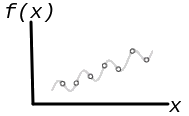
\includegraphics[scale=0.8]{figs/grafA.png}
        \label{fig:graf1:grafA} }
    \quad
    \subfloat[Hipótese linear]{
        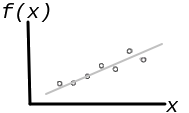
\includegraphics[scale=0.8]{figs/grafB.png}
        \label{fig:graf1:grafB} }
    
    \caption{Hipóteses ajustadas} \label{fig:graf1}
        
        %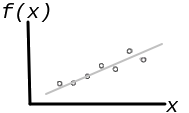
\includegraphics[scale=0.4]{figs/grafB.png}
        %\caption{Polinômio Superajustado} \label{grafB}
\end{figure}


O exemplo da figura \ref{fig:graf1:grafA} mostra uma função de grau 6 onde acontece  um sobreajuste (overfitting) no conjunto de dados de treinamento. Esse modelo acabou exibindo uma função mais complexa para atender todo o conjunto de dados do gráfico, ficando especifico para essa amostra. 

Já na figura \ref{fig:graf1:grafB} o ajuste da função se torna mais simples e mesmo o gráfico não passando por todos os pontos, acabou por generalizar melhor o conjunto de treinamento, tornando talvez, um melhor resultado da predição de novos valores. 

Em análise da figura \ref{fig:graf1} é apresentado duas hipóteses que tentam se aproximar ao máximo da função verdadeira (${h}$), que é desconhecida. Mesmo parecendo que  na figura \ref{fig:graf1:grafA} obteve-se melhor resultado, pois todos os pontos são atingidos pelo gráfico da função, este modelo acabou se ajustando muito bem na amostra de dados deixando a função ${h}$ muito específica, não retratando os dados em um mundo real. Então, apesar de parecer que a \ref{fig:graf1:grafA} por ser mais específica é a melhor função, não é a opção correta. Quanto mais  generalizado for modelo, melhor será para predizer os valores de ${y}$ para novos conjuntos de dados.

\subsubsection{Algoritmo Classification and Regression Trees  - CART}\label{cap:refTeor:sssec:cart}


Esse algoritmo constroi modelos de previsão a partir de dados de treinamento onde seus resultados podem ser reprensentados em uma árvore de decisão. A árvore de decisão é uma ferramenta que da suporte à decisão utilizando como modelo um fluxograma semelhante a uma árvore, onde a cada nó interno é feito um teste para tomada de decisão, permitindo uma abordagem do problema de forma estruturada e sistemática até chegar a uma conclusão lógica. ``Uma árvore de decisão alcança sua decisão executando uma sequência de testes'' \cite[p. 811]{RusselStuart.Norvig2013}

O algoritmo CART pode se tornar uma árvore de classificação ou também um árvore de regressão, o que irá definir seu tipo seria o atributo classe. Por exemplo, em um conjunto de dados de um paciente onde tenta prever se o mesmo possuirá câncer. A classe seria ``Terá Câncer'' ou ``Não terá Câncer''. Nesse exemplo o atributo assume duas classes.

Mas ao contrário de uma árvore de classificação que prediz uma classe, o CART também pode assumir uma árvore de regressão, onde poderá prever um valor numérico ou contínuo, como período de tempo de internação do paciente, preço de uma cirurgia ou quantidade de água ingerida. 

No caso de não ser probabilístico o grau de confiança em seu modelo de predição será embasada em respostas semelhantes em outras circunstâncias antes analisadas. 

Inicialmente todas as amostras se concentram no nó raiz, e a partir daí é apresentado uma questão, onde a intenção é separar o nó raiz em dois grupos mais homeogêneos. Dependendo da questão as amostras irão para a folha esquerda ou direita do nó raiz. O CART faz essa divisão em função da regra Gini de Impureza\footnote{O CART pode utilizar outros critérios de divisão de dados como: entropia e critério de Twoing} \cite{braiman1984}, e o índice Gini varia de 0 a 1, definindo o grau de pureza do nó. 

\begin{equation}
Gini(S)= 1 - \sum p^2(j/t)
 \label{eq:cartGini}
\end{equation}
Onde: ${p(j/t)}$ é probabilidade a priori da classe ${j}$ se formar no nó ${t}$. E ${S}$ é um conjunto de dados que contém exemplos de n classes
%\begin{itemize}
% \item ${S}$: é um conjunto de dados que contém exemplos de n classes
% \item ${p_j}$: é uma frequência relativa da classe ${j}$ em ${S}$
%\end{itemize}

Para construção de uma árvore existem três componente importantes \cite{yohannes1999classification}: 
\begin{itemize}
[noitemsep]
 \item Um conjunto de perguntas que servirá de base para fazer uma divisão;
 \item Regras de divisão para julgar o quanto é boa esta divisão;
 \item Regras para atribuir uma classe a cada nó;
\end{itemize}


% 
% \IncMargin{1em}
% \begin{algorithm}[h!]
% 
% \nl $melhorGini$; \tcc{cria a variável}
% \nl $divisaoCorrente \leftarrow 4.9$;\tcc{Ex. recebe o 1º valor do atributo} 
% \nl $direita \leftarrow 0$\; 
% \nl $esquerda \leftarrow 6$;\tcc{Ex. recebe o total de dados existentes para o atributo} 
% \nl \While{existirem dados}{
%  \nl \If{1ª Dado Lista do Atributo MAIOR $divisaoCorrente$}{ 
%       \nl $valorGini \leftarrow calculaGini(divisaoCorrente)$; 
%       } 
%  \nl \Else{ 
%         \nl$valorGini \leftarrow calculaGini(1ªDadoLista)$;
%         }
%  \BlankLine
%  
%  \nl \If{ Primeiro Gini encontrado}{
%         \nl $melhorGini \leftarrow valorGini$;
%         }
%     \nl \Else{
%         \nl \If{$valorGini > melhorGini$}{
%                 \nl $melhorGini \leftarrow valorGini$
%                 }
%             }        
%   \nl $divisaoCorrente \leftarrow 5.4$; \tcc{recebe o próximo dado do atributo}
%   \nl $direita$ recebe o que possui +1 e $esqueda$ o -1\;
%   \nl $(valorGini + divisaoCorrente)/2$;\tcc{encontrar ponto de divisão}
%  }
%  \caption{Rotina de funcionamento do CART com critério Gini \cite{Raimundo2008} }\label{alg:gini}
%  
% \end{algorithm}
% \DecMargin{1em}


\subsubsection{Algoritmo Naive Bayes}\label{cap:refTeor:sssec:nbayes}

É um modelo probabilístico que pode ser calculado diretamente entre seus dados de treinamento. Depois de calculado, o modelo pode ser utilizado para fazer previsões de novos dados através do teorema de Bayes. ``O teorema de Bayes fornece uma maneira de calcular a probabilidade de uma hipótese com base em sua probabilidade anterior, as probabilidades de observar vários dados, dadas as hipóteses, e os dados observados em si'' \cite[p. 156]{Mitchell1997}.



Esse teorema utiliza uma teoria estatística e probabilística para previsão de acontecimento de um evento, sendo este evento  relacionado a condição da probabilidade de ocorrência anteriores do mesmo. É nesse seguimento que o algoritmo Naive Bayes funciona. Criando classificadores  probabilístico baseados no teorema de Bayes.


Pode-se citar como exemplo desse evento, a descoberta do câncer em uma pessoa, pois se tal doença estiver relacionada ao sexo, então, utilizando o teorema de Bayes, o sexo de uma pessoa pode ser utilizada para da maior precisão a probabilidade de câncer, ao invés de fazer uma avaliação de probabilidade sem a utilização do sexo da pessoa.

O Naive Bayes utiliza uma técnica de independência dos atributos, onde cada variável de entrada não depende de recursos de outras. Essa independência condicionada  entre os atributos, os quais nem sempre ocorrem nos problemas reais, acabou deixando conhecida por Bayes ingênuo, ou Naive Bayes.

Em \citeonline{RusselStuart.Norvig2013} a equação \ref{eq:causaefeito} mostra a relação ${P(causa/efeito)}$ onde o efeito é evidência de alguma causa desconhecida, e quer se determinar a causa.

\begin{equation} \label{eq:causaefeito}
 P(causa|efeito)= \frac{P(efeito|causa)P(causa)}{P(efeito)}
\end{equation}

Naive Bayes como classificador estatístico possue um modelo de simples construção, e ficou conhecido por ter bons resultados em relação a algoritmos mais sofisticados, mesmo trabalhando com grandes quantidades de dados. Ele agrupa objetos de uma certa classe em razão da probabilidade do objeto pertencer a esta classe. 

\begin{equation}
 P(c/x)= \frac{P(x/c)P(c)}{P(x)}
\end{equation}

\begin{equation}
 P(c/x)=P(x_1|c)*P(x_2|c)*...*P(x_n|c)*P(c)
 \label{eq:bayes}
\end{equation}


\begin{itemize}
 \item ${P(c/x)}$ probabilidade posterior da classe ${c,alvo}$ dada preditor ${x,atributos}$.
 \item ${P(c)}$  é a probabilidade original da classe.
 \item ${P(x|c)}$  é a probabilidade que representa a probabilidade de preditor dada a classe.
 \item ${P(x)}$  é a probabilidade original do preditor.
\end{itemize}

A utilização do algoritmo Naive Bayes já é bem difundida, e está presente em vários trabalhos, como classificação de textos, filtro de SPAM, analisador de sentimentos, entre outros \cite{ Madureira2017, Lucca2013, Wu2008, Mccallum1997}. Mas mesmo atingido boa popularidade possui pontos negativos. A suposição de ter preditores independentes não acontece muito na vida real, pois acaba sendo difícil ter uma amostra de dados que sejam inteiramentes independentes. 


\subsection{Aprendizado Não-Supervisionado}\label{ssec:aprendNSup}

Outro cenário de aprendizado de máquina é o aprendizado não-supervisionado, onde nesse contexto não existe uma tentativa de se encontrar uma função que se aproxime da real. Logo porque os registros não são classificados, visto que o conjunto de treinamento não possui informação da saída sobre determinada entrada. Desta forma os algoritmos procuram algum grau de similaridade entre os registros e tentam agrupá-los de forma a ter algum sentido deles estarem juntos. 

Quando o algoritmo encontra dados com mesma similaridade ele os agrupa formando clusters. Os números de clusters encontrados dependerá do funcionamento dos algoritmos e também do grau de dissimilaridade entre elementos de grupos diferentes. Como não existe uma variável classe no aprendizado não-supervisionado, então segundo \cite{Barber2011}, o maior interesse seria em uma perspectiva probabilística de distribuição ${p(x)}$ de um determinado conjunto de dados.
\begin{equation}
 D = \{x_{n},n=1,...,N\}
 \label{eq:aprendNSup}
\end{equation}

Uma vez que no conjunto (\ref{eq:aprendNSup}), não existe classe ${y}$, encontrado em um conjunto de treinamento, equação \ref{eq:aprendSup}, o algoritmo precisa encontrar padrões nos atributos para fazer os agrupamentos.


\section{Discretização}\label{cap:refTeor:sec:discret}

O método de discretização faz a conversão de valores contínuos em valores discretos. A partir de um atributo com valores contínuos, a discretização cria um ponto inicial e final definindo um intervalo e designando uma faixa para cada intervalo. Assim, ao invés de valores contínuos os atributos possuiram novos contéudos no formato de faixas de valores.

Segundo alguns autores \cite{Catlett2006b,Hwang2002} a discretização melhora a precisão e deixa um modelo mais rápido em seu conjunto de treinamento. Os métodos de discretização mais comumente utilizados no âmbito dos métodos  não-supervisionados de acordo com \cite{Kotsiantis2006, Dougherty1995} são os métodos de Discretização por Larguras Iguais(EWD) e Discretização por Frequências Iguais (EFD).

%Aqui nesse trabalho é utilizado a técnica de discretização antes da execução dos algoritmos e as faixas selecionadas são usadas para identificar o rótulo. Após o conhecimento do rótulo o valor da faixa é trocado pelo início e fim do intervalo.



\subsection{Discretização por Larguras Iguais - EWD}\label{cap:refTeor:subsec:ewd}

O método de Discretização por Larguras Iguais (EWD) faz a discretização de um intervalo, entre valores contínuos, dividindo através de um ponto de corte as faixas de tamanhos iguais. Logo se existir um intervalo com valores contínuos [a,b], e deseja particionar em ${R}$ faixas de tamanhos iguais serão necessários ${R-1}$ pontos de corte, figura \ref{fig:pontocorte}. 

\begin{figure}[h]
        \centering
        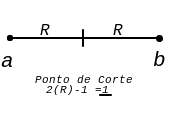
\includegraphics[scale=1]{figs/faixaA-B_PontoCorte.png}
        \caption{Ponto de Corte (R-1)} \label{fig:pontocorte}
\end{figure}

Para haver o ponto de corte antes tem que ser realizado a ordenação dos dados. A largura de cada faixa ${r_1,...,r_R}$ na equação \ref{eq:largurafaixa} é representada por ${w}$, que é calculada pela diferença entre os limites superior e inferior do intervalo, dividido pela quantidade ${R}$ de valores a serem gerados.

\begin{equation}
 w = \frac{b-a}{R}
 \label{eq:largurafaixa}
\end{equation}

A variável ${w}$ determina os pontos de corte ${(c_1,...,c_{R-1})}$ que irão delimitar o tamanho das faixas de valores. O primeiro ponto de corte, ${c_1}$, é obtido através da soma do limite inferior ${a}$ com a tamanho de ${w}$. E os pontos de corte seguintes são calculados pela soma do ponto de corte anterior com ${w}$.


O valor de cada faixa será representado por ${i}$, onde ${i}$ é o índice indicando a faixa. De acordo com a figura \ref{fig:faixasEWD} para dividir o intervalo ${[a,b]}$ em ${R}$ faixas será necessário de ${R-1}$ pontos de corte.

\begin{equation}
c_i=\left\{\begin{matrix}
a+w, & se\, i=1 & \\ 
c_{i-1}+w,  & caso\, contrário & 
\end{matrix}\right.
 \label{eq:regratamfaixa}
\end{equation}

O valor da faixa do intervalo ${[a,c_1]}$ será o valor discreto igual ao índice de sua faixa ${r_1}$. Então, um valor na faixa ${r_1}$ terá o valor reprensentado por ${1(um)}$, pois  ${i=1}$ é o limite inferior mais largura da faixa, equação \ref{eq:regratamfaixa}. E seguindo o mesmo raciocínio o valor da faixa ${r_2=]c_1,c_2]}$ é representado por ${2(dois)}$, e consequentemente o valor que se encontra em uma faixa qualquer ${r_i}$ será reprensentado por ${i}$.

%\afterpage{
\begin{figure}[h] 
        \centering
        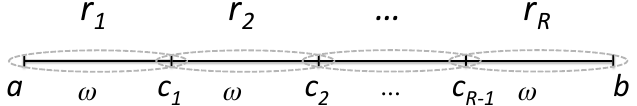
\includegraphics[scale=0.6]{figs/discretizacaoEWD.png}
        \caption[Discretização EWD]{Discretização EWD baseada em \cite{LOPES2014}}%\footnotemark } 
        \label{fig:faixasEWD}
\end{figure}
%\footnotetext{Figura extraída de \cite{Lopes}}
% }



\subsection{Discretização por Frequência Iguais - EFD}\label{cap:refTeor:subsec:efd}

Esse outro método de discretização já possui uma abordagem diferente a do EWD, pois a idéia é manter a quantidade de elementos distintos, entre os pontos de corte, com o mesmo número. Dado um intervalo ${[a,b]}$ o número de faixas ${R}$ e a quantidade de valores distintos ${\xi}$ , onde ${\xi \geqslant R}$ o método EFD irá segmentar em  ${R}$ faixas de valores que possuem a mesma quantidade de elementos distintos ${\lambda}$. Então serão realizados ${R-1}$ pontos de corte gerando ${R}$ faixas de valores, ${(r_1,...,r_R)}$, com a mesma quantidade de elementos distintos ${\lambda}$. Para encontrar ${\lambda}$ calcula-se o valor inteiro da divisão entre a quantidade de elementos distintos ${\xi}$ pela quantidade de faixas de valores ${R}$, obtendo o número de elementos da faixa \ref{eq:qtdelemfaixaEFD}.

\begin{equation}
\lambda = \frac{\xi}{R}
 \label{eq:qtdelemfaixaEFD}
\end{equation}

Uma observação nesse método é a ocorrência em amostras que possuem uma má distribuição de valores de um dado atributo. Como um número significativo de repetições, causando um desiquilíbrio nas distribuições dos elementos.

Uma vez no intervalo ${[a,b]}$ de elemetos ordenado e calculado ${\lambda}$ contendo ${R}$ elementos ${v_{[R]}}$  pode-se determinar os pontos de corte ${(c_1,...,c_{R-1})}$ que são os delimitadores das faixas. Cada ponto de corte ${c_i}$ pode ser calculado por ${v_{i\lambda}-ésimo}$ elemento, \ref{eq:pontocorteEFD}.

\begin{equation}
c_i = v_{[i\lambda]}
 \label{eq:pontocorteEFD}
\end{equation}

Igual o que aconteceu no método EWD, o valor que estiver no intervalo ${[a,c_1]}$ terá seu valor associado a um valor discreto igual ao índice ${i}$ de sua faixa ${r_i}$ conforme figura \ref{fig:faixasEFD}. Então, caso o valor esteja na faixa ${r_2}$ ele passará a ter o valor de seu índice ${i}$ igual a ${2(dois)}$. De maneira consecutiva os valores que estiverem na faixa ${r_3=]c_2,c_3]}$ terão valor ${3(três)}$. Uma outra observação desse método é que diferente do EWD, os intervalos podem assumir faixas com tamanhos diferentes.

%\afterpage{
\begin{figure}[h]
        \centering
        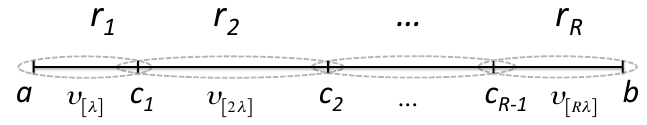
\includegraphics[scale=0.6]{figs/discretizacaoEFD.png}
        \caption[Discretização EFD]{Discretização EFD\footnotemark} 
        \label{fig:faixasEFD}
\end{figure} 
\footnotetext{Figura extraída de \cite{LOPES2014}}
%}


\section{Trabalhos Correlatos}\label{cap:refTeor:sec:trabcorrel}

Esta seção propõe relacionar outros trabalhos servindo de complemento teórico para entender a variedade de aplicações referente ao assunto de rotulação de dados.

O trabalho escrito por \citeonline{LOPES2014} fez um estudo abordando o tema de rotulação de dados, tema este, proposto também por esta pesquisa, mas com abrangência e execução diferentes do modelo da figura \ref{fig:modeloLOPES} . No trabalho de \citeonline{LOPES2014} foi utilizado como entrada um conjunto de dados onde foi feito o agrupamento automático, com algoritmos não-supervisionados formando  clusters. Logo após é utilizado um algoritmo supervisionado (Redes Neurais) nos grupos de dados, e apresentado como saída um rótulo específico que melhor define o grupo formado. Esses rótulos são formados pela faixa de valor, que mais se repetem, em conjunto com os atributos mais relevantes.

Pode-se verificar na figura \ref{fig:modeloLOPES} que na parte onde é aplicado o algoritmo supervisionado (processo III) é o local exato que esta pesquisa utiliza para testar outros algoritmos supervisionados, servindo para comprovar a hipótese desta proposta de mestrado.

\begin{figure}[h]
        \centering
        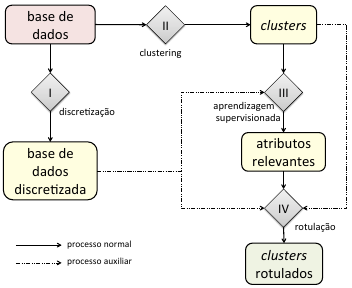
\includegraphics[scale=0.8]{figs/modeloLopes.png}
        \caption{Modelo \cite{LOPES2014}} 
        \label{fig:modeloLOPES}
\end{figure}


Em \cite{Metodo2015} o problema em questão é fazer classificação e rotulação em uma base que possuem poucos elementos classificados utilizando método semi-supervisionado. O método inicia com uma base dividida em elementos classificados(L) e não classificados(U). Após cada iteração o grupo L vai crescendo e automaticamente diminuindo o grupo U até que não tenha mais nenhum elemento em U, figura  \ref{fig:modeloVicente}. Após isso é realizado uma etapa de agrupamento, sem levar em consideração os dados classificados anteriormente. Terminada essa etapa é feito uma validação para saber quais os rótulos foram considerados corretos.
\begin{figure}[!h]
        \centering
        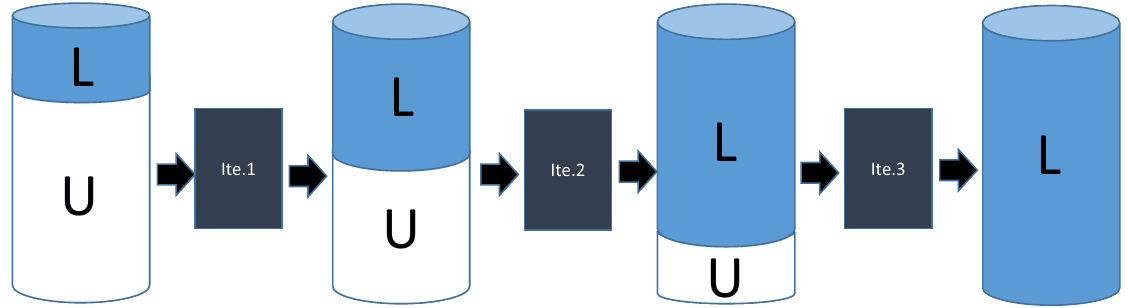
\includegraphics[scale=0.4]{figs/modeloVicente.png}
        \caption{Comportamento da base de dados a cada iteração. Método \cite{Metodo2015}} \label{fig:modeloVicente}
\end{figure}

O método proposto é uma combinação de um classificador com um método de agrupamento, onde a rotulação de um conjunto de dados é feita com conhecimento prévio de um outro conjunto menor rotulado. O classificador treina com a parte de dados rotulada e classifica os dados não-rotulados.


Outra pesquisa sore rotulação está em \cite{Filho2015} onde aborda o mesmo Problema de Rotulação, mas a atuação é diferenciada, pois o modelo procura diferenças existentes em cada grupo através da seleção dos elementos que representam o grupo, e depois é construído a faixa de valores. Os grupos são formados pelo algoritmo Fuzzy C-Means e após isso que é selecionado os atributos. 
% \begin{figure}[!h]
%         \centering
%         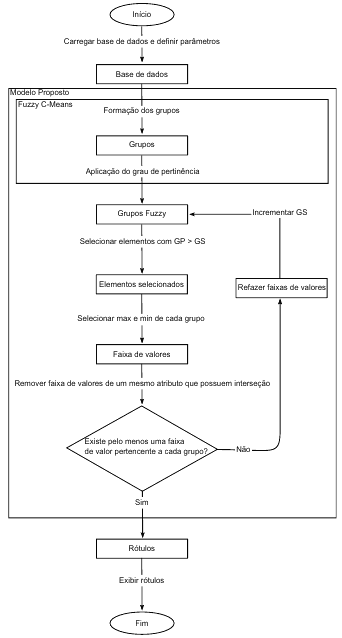
\includegraphics[scale=0.8]{figs/modeloRotFuzzy.png}
%         \caption{Modelo \cite{Filho2015}} \label{fig:modeloFilhoVilmar}
% \end{figure}






